\chapter{The Physics of Gases}

The air you breathe is a blend of gases:
\begin{enumerate}
\item 78\% nitrogen in the form of $N_2$
\item 21\% oxygen in the form $O_2$
\item 1\% other gases (mostly argon)
\end{enumerate}

If you fill a balloon with helium ($He$),  the helium will push against the interior of the balloon with some pressure.   
The pressure is the same at every point in the interior of the balloon.  Pressure,  then,  is force spread over some area.   
Force is commonly measured in newtons.   Pressure is measured in \newterm{pascals}.  A pascal is 1 newton per square meter.

We don't usually think about it,  but the air outside the balloon is also pushing against the exterior of the balloon.  
We call this \newterm{barometric pressure}, and it is caused by gravity pulling on the gas molecules above the balloon.

Imagine a square meter on the ground at sea level.  Now imagine the column of air above it -- reaching all the way to the top of the atmosphere.   
The air inside that column has a mass of about 10,340 kg.  One kilogram on the earth experiences a gravitational force of 9.8 N.   
So the atmospheric pressure (also called \newterm{barometric pressure} all around you is about 101,332 pascals.  
When dealing with such large numbers, we often use kilopascals.  
We'd say the barometric pressure at sea level is about 101.3 kPa.

We live pretty much oblivious to this huge force that is all around us, but you can see it sometimes.  
For example, if you suck the air out of a plastic bottle,   the bottle will be crushed by the barometric pressure.

\section{Altitude and Atmospheric Pressure}

If you let go of the balloon, as it rises through this column there will be less and less air pressure on the outside 
of the balloon and the balloon will expand.   What would be the atmospheric pressure at $h$ meters above sea level?  Here is a handy formula for that:

$$p = 101,332 \times \left(1 - \left( 2.25577 \times 10^{-5} \times h\right) \right)^{5.25588}$$

where $p$ is the atmospheric pressure in pascals.

\begin{Exercise}[title={Atmospheric Pressure},  label=atmos_pressure]
  
You are thinking about riding your bicycle to the top of Mount Everest.  You are worried when the atmospheric pressure outside the tire drops,  the tire will fail.  
(This has happened to me; It is very, very loud.)  

Calculate the atmospheric pressure at the top of Mount Everest (9,144 meters above sea level).

\end{Exercise}
\begin{Answer}[ref=atmos_pressure]

$$p = 101,332 \times \left(1 - 2.25577 \times 10^{-5} \times h\right)^{5.25588}$$

and $h = 9,144$.  Thus,

$$p \approx 30.1 \text{kPa}$$

\end{Answer}

\section{The Temperature of a Gas}

Now,  let's say you start to heat the helium inside the balloon.  As the temperature goes up,  the molecules inside will start to move faster.

Remember that the kinetic energy of an object with mass $m$ and velocity $v$ is given by

$$k = \frac{1}{2} m v^2$$

So, you could say "As the temperature of the gas increases,  the kinetic energy of the molecules increases."

To a physicist, however, the kinetic energy of the molecules and the temperature of the gas \emph{are the same thing}.  
That is, when you say "Balloon A, filled with helium, is the same temperature as Balloon B, which is filled with $H_2$"  
you are really saying "The average kinetic energy of a molecule in Balloon A is the same as the average kinetic energy of a molecule in Balloon B."

(In this example,  a helium molecule is about twice as heavy as an $H_2$ molecule.   Look at the formula for kinetic energy.
The molecules in Balloon B have to be generally moving faster than the molecules in Balloon A.)

\subsection{A Statistical Look At Temperature}

If you say "This jar of Argon is 25 degrees Celsius,"  you have told me about the \emph{average} kinetic energy of the molecules in the jar.  
However,  some molecules are moving very slowly.  Others are moving really,  really fast. 

We could plot the probability distribution of the speeds of the molecules.  For Argon at 25 degrees Celsius, it would look like this:

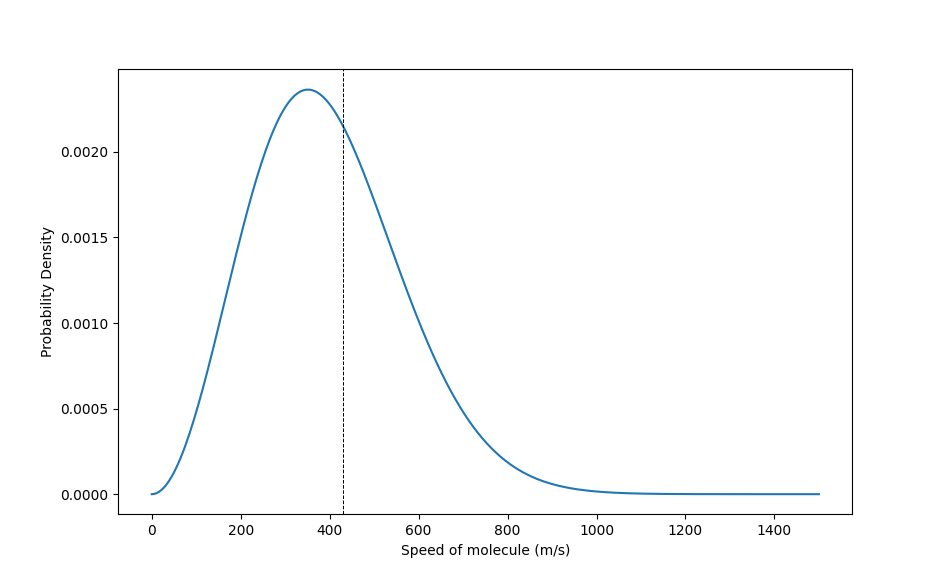
\includegraphics[width=\textwidth]{ar_plot.png}

The temperature,  remember,  is determined by the average kinetic energy of the molecules.  Some molecules are moving slowly and have less kinetic energy than the average.  Some molecules are moving very quickly and have more kinetic energy.  The dotted line is the divider between the two groups: molecules moving at speeds to the left of the line have less kinetic energy than average; those on the right have more kinetic energy than average.

Where is that line?  That is the RMS of the speeds of the molecules.  That is, if we measured all the speeds of all the molecules  $s_1, s_2, s_3, \ldots, s_n$, that line would be given by the root of the mean of the squares:

$$v_{rms} = \sqrt{\frac{1}{n} \left( s_1^2 + s_2^2 + s_3^2 + \ldots s_n^2 \right)}$$

If you have the same gas at a lower temperature, the distribution shifts toward zero:

Here is probability distribution of molecular speeds for argon gas at 25 degrees and -100 degrees Celsius.

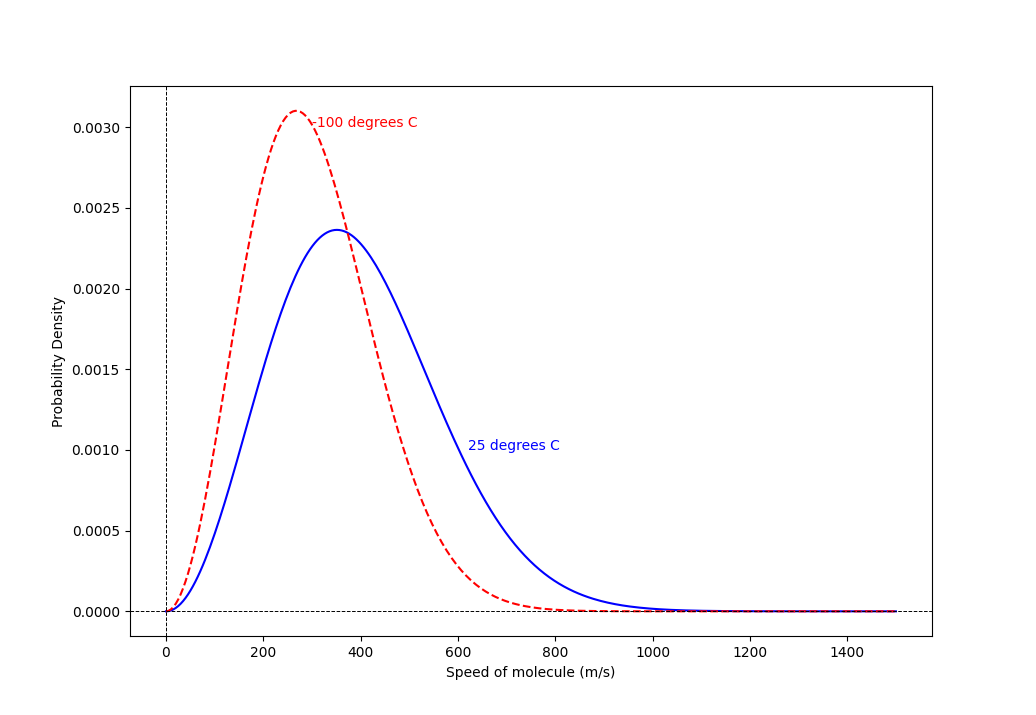
\includegraphics[width=\textwidth]{ar2_plot.png}

If you keep lowering the temperature,  eventually the molecules stop moving.  This is known as \newterm{absolute zero} -- you
 can't make anything colder than absolute zero.   Absolute zero is -273.15 degrees Celsius.
 
Besides Celsius and Fahrenheit, there is a third temperature system: Kelvin.  The Kelvin has the same scale as Celsius, but it starts at absolute zero.   
So,  0 degrees Celsius is 273.15 degrees Kelvin.    And 100 degrees Celsius is 373.15 degrees Kelvin.

Any time you are working with the physics of temperature, you will use Kelvin.

Let's say you have a half-full air mattress in a field with a person lying on it around dawn.   The weight of the person will keep the pressure of the air inside constant (or pretty close).  
The molecules in the mattress are not entering or leaving that mattress.  However, as the sun rises,  the air inside will get warmer and expand.  The person will be gently lifted by the expanding air.  How much will the air expand?

If you have constant pressure and number of molecules,  the volume of the gas is proportional to the temperature in Kelvin:

$$V \propto T$$

\begin{Exercise}[title={Temperature and Volume},  label=temp_vol]
  
At dawn, the air inside mattress at dawn has a volume of 1000 liters and a temperature of 12 degrees Celsius.

At noon,  that same air has a temperature of 28 degrees Celsius.  The pressure on the gas has not changed at all.

What is the volume of the gas at noon?

\end{Exercise}
\begin{Answer}[ref=temp_vol]

First, we convert the temperatures into Kelvin:  
\begin{enumerate}
\item Dawn: $12 + 273.15 = 285.15$
\item Noon: $28 + 273.15 = 301.15$
\end{enumerate}

So, the temperature $T$ has increased by a factor of $\frac{301.15}{285.15} \approx 1.056$

Thus the volume of the air mattress has also increased by a factor of 1.056.  

So the air mattress that had a volume of 1000 at dawn,  will have a volume 1056 at noon.

\end{Answer}

Note: Volume and temperature are only proportional as long as the substance is a gas.   We will talk about liquids and solids soon.






